\documentclass[border=8pt]{standalone}
\usepackage[T1]{fontenc}\usepackage[utf8]{inputenc}\usepackage{lmodern}
\usepackage{tikz}\usetikzlibrary{arrows.meta,positioning}
\begin{document}
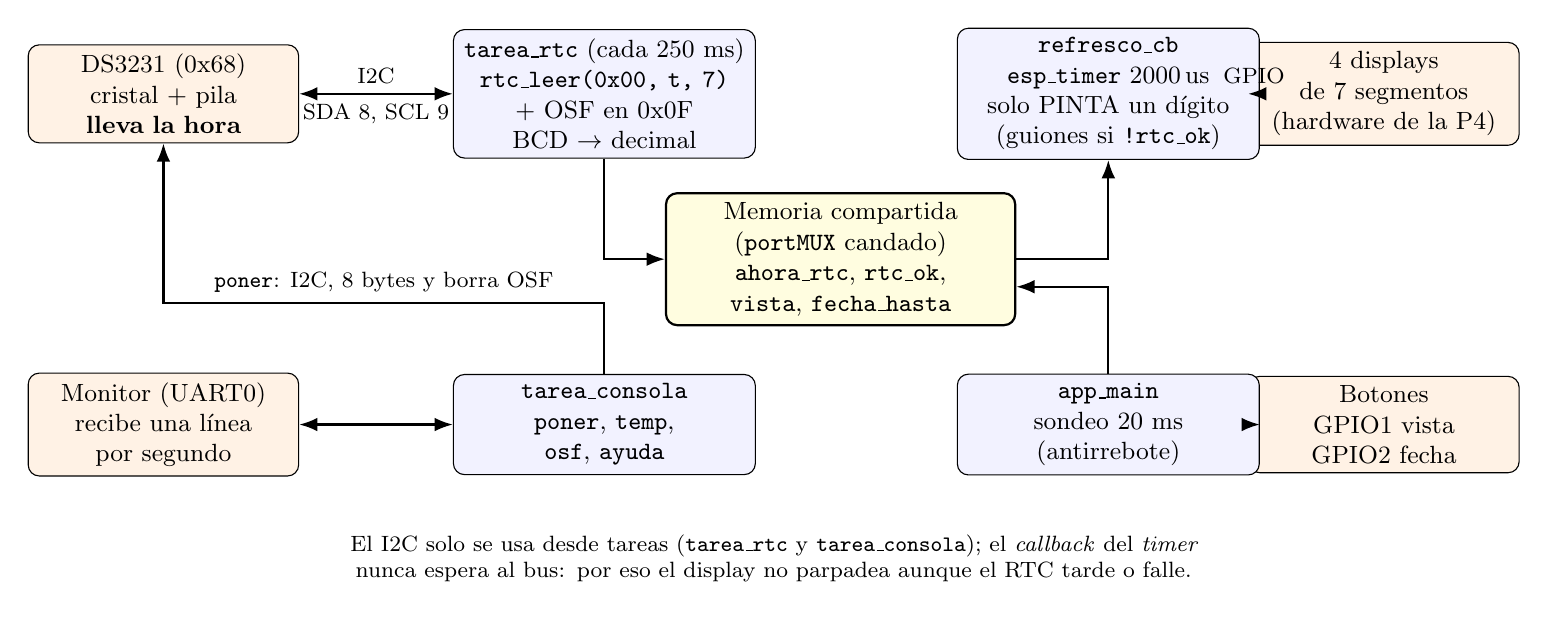
\begin{tikzpicture}[>=Latex,font=\small,
 b/.style={draw,rounded corners,fill=blue!5,align=center,minimum height=1.2cm,text width=3.6cm},
 h/.style={draw,rounded corners,fill=orange!10,align=center,minimum height=1.2cm,text width=3.2cm},
 m/.style={draw,thick,rounded corners,fill=yellow!12,align=center,minimum height=1.2cm,text width=4.2cm}]
% hardware
\node[h] (rtc) at (0,0) {DS3231 (0x68)\\cristal + pila\\\textbf{lleva la hora}};
\node[h] (dsp) at (15.5,0) {4 displays\\de 7 segmentos\\(hardware de la P4)};
\node[h] (btn) at (15.5,-4.2) {Botones\\GPIO1 vista\\GPIO2 fecha};
\node[h] (mon) at (0,-4.2) {Monitor (UART0)\\recibe una línea\\por segundo};
% software
\node[b] (trtc) at (5.6,0) {\texttt{tarea\_rtc} (cada 250 ms)\\\texttt{rtc\_leer(0x00, t, 7)}\\+ OSF en 0x0F\\BCD $\to$ decimal};
\node[m] (mem) at (8.6,-2.1) {Memoria compartida\\(\texttt{portMUX} candado)\\\texttt{ahora\_rtc}, \texttt{rtc\_ok},\\\texttt{vista}, \texttt{fecha\_hasta}};
\node[b] (ref) at (12.0,0) {\texttt{refresco\_cb}\\\texttt{esp\_timer} 2000\,us\\solo PINTA un dígito\\(guiones si \texttt{!rtc\_ok})};
\node[b] (app) at (12.0,-4.2) {\texttt{app\_main}\\sondeo 20 ms\\(antirrebote)};
\node[b] (con) at (5.6,-4.2) {\texttt{tarea\_consola}\\\texttt{poner}, \texttt{temp},\\\texttt{osf}, \texttt{ayuda}};
\draw[<->,thick] (rtc) -- node[above,font=\footnotesize]{I2C} node[below,font=\footnotesize]{SDA 8, SCL 9} (trtc);
\draw[->,thick] (trtc.south) |- (mem.west);
\draw[->,thick] (mem.east) -| (ref.south);
\draw[->,thick] (ref) -- node[above,font=\footnotesize]{GPIO} (dsp);
\draw[->,thick] (btn) -- (app);
\draw[->,thick] (app.north) |- ([yshift=-0.35cm]mem.east);
\draw[<->,thick] (mon) -- (con);
\draw[->,thick] (con.north) -- ++(0,0.9) -| node[pos=0.25,above,font=\footnotesize]{\texttt{poner}: I2C, 8 bytes y borra OSF} (rtc.south);
\node[font=\footnotesize,text width=18cm,align=center] at (7.75,-5.9) {El I2C solo se usa desde tareas (\texttt{tarea\_rtc} y \texttt{tarea\_consola}); el \emph{callback} del \emph{timer} nunca espera al bus: por eso el display no parpadea aunque el RTC tarde o falle.};
\end{tikzpicture}
\end{document}
